\documentclass[10pt,a4paper]{article}
\usepackage[utf8x]{inputenc}
\usepackage{ucs}
\usepackage{amsmath}
\usepackage{amsfonts}
\usepackage{amssymb}
\usepackage{apacite}
\usepackage{graphicx}
\usepackage{url}
\usepackage{parskip}

\author{Kristjan Valur Jonsson}
\title{TSense Authentication Protocols\\Working Draft}


\begin{document}

\maketitle

\begin{abstract}
This document describes some ideas for TSense authentication and transport protocols. The system architecture is outlined and the protocols informally analyzed.
\end{abstract}


\section{System sketch}

The basic system is shown in its simplest form in Figure~\ref{fig:sys-overview}. The players are:
\begin{description}
\item \textbf{Trusted sensor ($T$)} measures some array of quantities, e.g.\ temperature, pollutant particle count and luminosity, and publishes in an authenticated manner to a client ($C$). The published results may additionally be encrypted.
\item \textbf{Client ($C$)} hosts the sensor, e.g.\ physically attached or USB-connected. The client is the corruptable (adversary controlled) entity in our model. The purpose of $C$ is to participate in a measurement network, either honestly or in such a manner that its actions are indistinquishable from that of a honest client. A honest client will always forward measurements unmodified to the sink $S$, whereas a corrupted $C$ may modify all or individual readings. We simplify our present model so that each $C$ hosts exactly one sensor $T$. Further, each $C$ communicates directly with exactly one sink/clusterhead $S$.
\item \textbf{Sink ($S$)} collects measurements forwarded from the client. A network may include multiple networked sinks, in which each of the sinks is a \textit{clusterhead} for a number of clients. In this work, we regard all $S$ to be trusted -- that is, while some ratio $n/k$ of $k$ clusterheads to $n$ clients (sensor nodes) may be maintained for reasons of scalability, we regard the collection $C$ to be incorruptible. This is a simplifying assumption that will be relaxed in future work.
\item \textbf{Authentication service ($A$)} handles authentication of sensor nodes and clients at time of insertion into a working measurement network. Even though we regard the $S$ to be trusted, it is a prudent measure to limit distribution of sensor keys. In our model, we limit the distribution of the private sensor keys to only the sensor $T$ and the $A$\footnote{Recall that we use a shared private key issued at the time of manufacture, primarily for reasons of efficiency. Public key crypto would ease the key distribution issues, but is more computationally intensive. We therefore opted to use only symmetric cryptographic primitives in our prototype.}. We regard $A$ to be incorruptible (unconditionally). A single $A$ is assumed, which is a somewhat reasonable assumption from a scalability standpoint, since authentication takes place much less frequently than data collection. A single $A$ is of course a single point of failure, but in our model, we are primarily concerned with stealthy attacks, rather than noisy attacks, like DDoSing the authentication service.
We assume the authentication service $A$ is accessed only by $s \in S$, and never directly by any $c \in C$. This simply limits the exposure potential of $A$ to adversaries. In this project, we implicitly assume perfect mutual trust between any $s$ and $A$. In reality, measures would have to be taken to harden $A$, but this task is eased by limiting the population of nodes which have access to it. All communications between $A$ and $s_j$ are encrypted, as a TLS/SSL tunnel and mutual authentication assumed. Additionally, we can use asymmetric crypto to add a further layer of security to the exchange.
\end{description}

\begin{figure}
\begin{center}
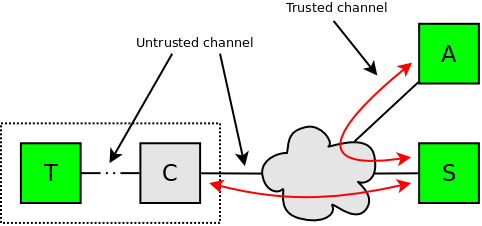
\includegraphics[width=0.6\textwidth]{figures/sys-overview.png} 
\end{center}
\caption{System overview. Interaction of the entities of the system. Green: Trusted entities. Gray: Untrusted entities (compromizable), Black channels: Insecure, Red channels: Secure.}
\label{fig:sys-overview}
\end{figure}

All channels are regarded as untrusted. However, protection against outsider adversaries is assumed to be prevented by standard cryptographic primitives -- pre-shared secret keys, or asymmetric crypto-based key negotiation\footnote{We use SSL/TLS to wrap this in our implementation.} as appropriate.


\section{Security requirements}

Attacker model: The attacker model is fairly simple. One or more adversaries can each corrupt one or more clients. All clients under the control of a given adversary can collude to influence measurements forwarded from a hosted sensor. The goal is to prevent the corrupt entities (within computational bounds) from \textit{forging} fictious messages -- generating false measurements which are accepted by the corresponding sink.
Sensors $T$, sinks $S$ and the authentication server $A$ are considered trusted in the current work.

\begin{itemize}
\item \textbf{$T$ must be uniquely identified to $A$.} Cloning or simulation of sensors must be prevented. No sensor may be in operation on multiple sinks at any given time.
\item \textbf{$A$ must vouch for the authenticity of a given $T$ to a given $S$.} 
\item \textbf{The authenticity of a sink $S$ must be proven to a given $T$ at time of insertion.} The sink with which the $T$ is communicating must be a member of an authorized group of sinks. This requirement may be relaxed s.t.\ any given $S$ is accepted by any given $T$, but is easy to enforce by the fact that only authorized $S$ are able to contact $A$ and complete the authentication protocol.
\item \textbf{The integrity of sensor data must be protected} s.t.\ an attacker (corrupted $C$) is reduced to simulate crash failure (neglect forwarding updates) in order to influence the ultimate aggregate computation.
\item \textbf{The confidentiality of sensor data may optionally be protected} s.t.\ a hosting $C$ or an eavesdropper is prevented from learning the contents of the messages. A side effect of encryption is that the task of the attacker is made more difficult: its ability to make intelligent choices as to which updates to drop is effectively removed.
\item \textbf{A $S$ must only accept measurements from an unique instance of a valid $T$.}
\end{itemize}

\textbf{A note on crash failure simulations (omissions). We can for example limit the attackers ability to drop packets by policies on allowable dropouts. A client producing erratic results can be banned temporarily from the system. Some sort of reputation mechanism can be applied here. We will not explore this subject further in this work and simply regard the crash-failure-only behavior of corrupted entities to be sufficient for our purposes.}

\section{Symmetric authentication and key exchange protocol}

This section outlines a very basic symmetric authentication protocol, using a trusted server $A$. It is based on the Needham-Schroeder authentication and key exchange protocol \shortcite{needham1978} [B. Schneier -- Applied Crypto]. A modified Needham-Schroeder is also used in the Kerberos protocol \shortcite{neuman1994}. The main modification in our protocol is that $T$ does not communicate directly with $A$ but through $S$. This adds a layer of obscurity to $A$ as only the fairly well trusted $S$ need direct knowledge of its address.

The original Needham-Schroeder was vulnerable to replay attacks \shortcite{denning1981}, which can be fixed by using nonces and/or timestamps \cite{needham1987}. We use nonces to prevent replays.

The first messages in the protocol are similar to the YubiKey\footnote{\url{http://www.yubico.com/products/yubikey}} \shortcite{merkel2009} one-time password authentication protocol. However, the YubiKey protocol is not a key exchange protocol, but rather constructs a verifiable one-time secret. In essence, the YubiKey packet boils down to
\[
token = [T_{pub},T_{pr},N_T,CRC]
\]
which is similar to an encryption of the first message produced by $T$ in our protocol. The nonce used by the YubiKey protocol consists of two separate counters, a timer field and a random number -- the complicated (and long) nonce really adds no entropy if a strong block cipher is used. This is similar to the first encrypted token passed from $T$ to $C$.

\subsection{The authentication mode}

We use the \textit{Encrypt-then-MAC (ETM)} method of \shortciteA{bellare2007} in which the plaintext is first encrypted and then a MAC of the ciphertext appended:
\[
\mathcal{E}_{K_e \parallel K_a} = \mathcal{E}_{K_e}(M) \parallel \mathcal{T}_{K_a}(C)
\]
where
\[
C = \mathcal{E}_{K_e}(M)
\]
This construction is proven more secure than the other two generic compositions (encrypt-and-MAC and MAC-then-encrypt) by \citeauthor{bellare2007}. $ \mathcal{T}$ is here a MAC operation with a symmetric key $K_a$.

\subsection{Authentication and session key exchange protocol}

The authentication and session key exchange proceeds as follows:
\[
C \rightarrow T: \textit{queryId}
\]
The client $C$ (untrusted) queries the sensor $T$ for its public ID.

\[
T \rightarrow C: (T,\mathcal{E}_{TA}(T,N_T) \parallel \mathcal{T}_{TA,a})
\]
The sensor $T$ returns its public id and an encryption of its public id with a nonce using the secret key $K_{TA}$. The whole thing is MACed for authenticity -- we denote this from here on by the symbol $\mathcal{T}$. This message is very similar to the YubiKey OTP. The nonce is only sent in encrypted form in this construction. Its purpose is to prevent replay attacks (provide freshness). The eventual recipient of the encrypted payload (the authentication server $A$) checks the nonce for consistency and returns with the eventual reply to $T$.

\[
C\rightarrow S: (insert,T,\mathcal{E}_{TA}(T,N_T) \parallel \mathcal{T}_{TA,a})
\]
$C$ passes the public id of $T$ and the encrypted packet to $S$.

\[
S \rightarrow A: (\mathcal{E}_{AS}(insert,T,N_S, \{ \mathcal{E}_{TA}(T,N_T) \parallel \mathcal{T}_{TA,a} \}) \parallel \mathcal{T}_{AS,a})
\]
$S$ forwards the sensor public ID $T$, own nonce $N_S$ to $A$ and unmodified encrypted payload to $A$. $A$ checks if $T$ is on record, and if so, generates response. A non-existent id should probably log the $S$ as a possible attacker. 
%
$S$ forwards the encrypted/authenticated packet from $T$ unmodified to $A$, but adds extra security by encrypting by a pairwise shared key $K_{AS}$ and authenticating with the derived shared key $K_{AS,a}$. This can most directly be accomplished by using mutually authenticating TLS to set up these keys and provide the crucial identification of the two trusted entities $A$ and $S$.

\[
A \rightarrow S: (\mathcal{E}_{AS}(OK,N_S,K_{ST},t_{ST}, \{ \mathcal{E}_{AT}(N_T,K_{ST},t_{ST}) \parallel \mathcal{T}_{AT,a} \} \parallel \mathcal{T}_{AS,a})
\]
A responds with a code for OK (else, returns error code). The nonce $N_S$ is included, along with a randomly generated session key $K_{ST}$ and expiration "time" $t_{st}$ of some sort\footnote{We have to think about this a bit since the Arduino has no real time clock and we want to avoid depending on $C$ for time synchronization. A counter decremented per usage or simply a timelimit in seconds should be ok. Another option is to ignore this for the time being.}. $A$ also embeds an encrypted package for $T$, containing the session key $K_{ST}$, MACed for authenticity. The shared symmetric key $K_{AT}$ and the original nonce $N_T$ provide guarantees to $T$ that it was in fact $A$ that generated this key.

\[
S \rightarrow C \rightarrow T: (\mathcal{E}_{AT}(N_T,K_{ST},t_{ST}) \parallel \mathcal{T}_{AT,a})
\]
$S$ forwards the encrypted package containing the nonce and session key to $T$ through $C$. $T$ opens the package and retrieves $K_{ST}$. 

Note: The session key $K_{TS}$ is a fairly long term \textit{ephemeral} key. See motivation for use of ephemeral keys in e.g.\ Menezes (pp.\ 494). $T$ and $S$ also derive an authentication key $K_{TS,a}$ at this point.

\subsection{Initial encryption key establishment}

The session key has now been delivered to $T$ and $S$. Needham-Schroeder includes a handshake step in which the entities receiving the session key make sure they both have the correct key. We also use the handshake for the initial exchange of encryption/authentication keys. These are the keys which are used in the bulk of the crypto operations -- the data transfer itself.

The handshake/key exchange must happen right after the delivery of $K_{ST}$ to $T$ and then periodically to refresh the encryption and authentication keys. See also Menezes (pp.\ 497) on point-to-point key update.
\[
T \rightarrow C \rightarrow S: (\textit{re-key},T,\mathcal{E}_{ST}(T,N_T) \parallel \mathcal{T}_{ST,a})
\]
$T$ uses the session key $K_{ST}$ to request a fresh key. In the first round, this message also serves to let $S$ know the session key $K_{ST}$ was successfully delivered. $N_T$ is a new nonce.

\[
S \rightarrow T: (\textit{new-key},T, \{ \mathcal{E}_{ST}(T,N_T,R,t_{expire}) \parallel \mathcal{T}_{STe,a} \} )
\]
$S$ returns a fresh random number $R$ to $T$ (the new key material). $t_{expire}$ is the expiration "time" -- actually, we can use a counter for this so that $T$ requests a new key when the counter reaches zero. The encryption key is derived from this as $K_{STe}=\mathcal{E}_{ST}(R)$. The purpose of this step is to provide bilateral implicit key authentication (See Menezes pp.\ 498). Better yet, use a one-way cryptographically secure hash function for this derivation instead of encryption (see later section on key derivation). $S$ considers the session officially to have been established once the initial encryption key has been delivered.

%Note: All $AS$ communications are implicitly encrypted over the SSL tunnel. We can therefore simplify the communications between those entities considerably. $AS$ encryption and authentication included in the protocol above for completeness only.

%Note: MACs are used pretty liberally in the protocol shown, perhaps excessively. If space (bitsize) is an issue, we can truncate a long MAC to any size that still retains reasonable security. Of course, an authenticated encryption mode would make most of the MACs unnecessary.

\subsection{Subsequent re-keying}

How will $T$ request keys in the future when its keys expire, since it is totally dependent on $C$ for outside communication? One way is to add a control message, like the re-keying message above, to the measurement queue which a well-behaved $C$ will forward. $T$ will then simply not produce any output until a new key is delivered. A $C$ meddling with the re-keying would then simply produce no (verifiable) output.

The encryption and authentication keys $K_{TSe}$ and $K_{TSe,a}$ used for the actual traffic are short term \textit{ephemeral} keys, good for a very limited amount of traffic, say 10000 encryptions.

\subsection{Finish message}

A well-behaved client should send a \texttt{FINISH} message when it wishes to terminate a session. This message could carry some summary of the session, e.g.\ start, end times and total number of messages sent, allowing the server to do some sanity checks (see TLS for reference). A FINISH message will invalidate the current $S$-side session and encryption keys and clean up resources. 

However, clients may leave without any notice. We must handle that by using a soft-state on the $S$ -- a keep-alive timer is reset each time an update is received from a client and the session keys invalidated once the timer elapses.

Note: This refers to the key state only. Actual network connections can be opened per transaction.


\section{Transfer protocol}

The transfer protocol uses the encryption and authentication keys and is pretty straight forward. The following is a pull-based protocol but a push based is a simple modification.

\[
C \rightarrow T: (\textit{poll})
\]
$C$ requests the current measurements from $T$. Alternatively, we let $T$ push the measurements and skip this step.

\[
T \rightarrow C \rightarrow S: (\textit{update},T,N_T,\mathcal{E}_{STe}(T,N_T,B) \parallel \mathcal{T}_{STe,a})
\]
T (optionally) encrypts the buffer $B$, MACs and delivers to $C$, who simply forwards the packet to $S$. A nonce $N_T$ prevents replays -- can simply be a monotonic counter incremented during the lifetime of the encryption key.

The message contents $B$ can for example be of the following form:
\[
[length \parallel r_1 \parallel \dots \parallel r_n ]
\]
where length is the total length in bytes and $r_i$ is a record:
\[
r_i = [interface name \parallel timestamp \parallel value ]
\]

Note: If $B$ is sent in plaintext then we use a MAC over the plaintext, rather than cipher text. That is, simply skip the encryption step.

Note: The encryption and authentication keys $K_{STe}$ and $K_{STe,a}$ must be replaced periodically by a re-keying operation, as discussed previously.

\section{Handling the unexpected}

The protocols outlined above assume well-behaved participants. This is not necessarily the case. We have to think about and handle the problems that can occur -- check on nonces, IDs and so forth. We also have to maintain a soft state for all stages in the protocol and enforce some time limit on steps -- a client or any other node taking too long would cause the protocol to be aborted.


\section{Keys and key derivation}

A number of keys are used in the authentication and session keying protocols with the ultimate goal of establishing the encryption and authentication keys used in the transfer protocol. The keys and their derivation functions are summarized in this section.

The keys used are the following:

$K_{TA}$ is the secret identity of the sensor $T$. It's unique for each sensor and shared only with $A$. An authenticity key is derived from $K_{TA}$: $K_{TA,a} = f_{TA,a}(K_{TA})$. The permanent secret keys are only used for initial authentication.

$K_{AS}$ and $K_{AS,a}=f_{AS,a}(K_{AS})$ are the shared keys for $S$ and $A$. These can be established using SSL/TLS and the necessary strong mutual authentication of these trusted entities. We assume $S$ and $A$ have digital certificates and negotiate these keys regularly, at least on every connection.

$K_{ST}$ and $K_{ST,a}=f_{ST,a}(K_{ST})$ are the session encryption and authentication keys, shared between $S$ and $T$. The key is generated (a random number is sufficient) by $A$ on successful identification of $T$. The session key is used only for re-keying and perhaps some controlling -- very sparingly.

$K_{STe}$ and $K_{STe,a}=f_{STe,a}(K_{STe})$ are the actual encryption and authentication keys. They have a limited lifetime and must be replaced periodically by performing the re-keying protocol. If authentication-only mode is used, we simply skip deriving the corresponding encryption key $K_{STe}$.

The function $f$ can be a cryptographically secure hash function, in which case the derivation is essentially $K_a = f(K \parallel \alpha)$, similar to the key derivation function KDF1 in IEEE-1363-2000 \cite{ieee-1363-2000}. We have a keyed cryptographically secure hash function available, that is CMAC, so we might as well use that. In that case, we have $K_a = MAC_{\alpha}(K)$. $K$ is here the "key material" -- a base key or shared random value. In both cases, $\alpha$ is a pre-defined constant for each type of key produced. We can iterate the operation several times, similar to whats done in \shortcite{rsa-pkcs5-v2-1999}, but once is probably sufficient for our purposes. The output of the hash function or MAC is truncated down to the cryptographic key length. See also Menezes (ch. 13) on key derivation.


\section{The "certificate" of $T$}

Each individual $T$ has embedded unmodifiable information, which we call its certificate.

\begin{itemize}
\item \textbf{Public ID} is a concatenation of a globally unique manufacturer ID (2 bytes) and a per-manufacturer unique serial number (4 bytes). The interface for the sensor must include a function to retrieve this information.
\item \textbf{Private ID} is a random number selected by the manufacturer at assembly time (128-bits). Also known as the permanent secret key $K_{TA}$, where $T$ is a sensor device and $A$ is a manufacturer. This key is never revealed to anyone, except indirectly (by using it to encrypt) to $A$.
\item \textbf{Manufacturer Information} is plaintext information which includes: 
\begin{itemize}
\item Manufacturer name
\item Address
\item Website
\item Sensor model, version.
\item Assembly date
\item Serial number
\end{itemize}
The interface for the sensor must include a function to retrieve this information.
\item \textbf{Manufacturer "signature" for plaintext identifying information}. A MAC of a hash of the plaintext info, computed using a key derived from the master shared secret key.
\end{itemize}


%\section{Zero-knowledge authentication and key exchange}

%It would certainly be beneficial to reduce the reliance on a single $A$ for authentication, even if only for the reason of a single point of failure and potential congestion. 

%In our scheme, the $S$ clusterheads could cache the public keys for sensors (the certificates) or request on demand. The importance of and reliance on $A$ would be greatly reduced. In fact, we could reasonably get away with implementing it at all in our simple 3 node system. We would require at least a honest verifier zero knowledge protocol.


%The problem is that a pure zero-knowledge protocol requires asymmetric crypto.

%Feige-Fiat-Shamir -- see \cite{castelluccia2004} on an efficient variant.

%Guillou-Quisquater \shortcite{guillou1988} suitable for smartcards.

%Schnorr \shortcite{schnorr1989} and Okamoto \shortcite{okamoto1993} (improvement of Schnorr) also suitable for smartcards. Schnorr's ID scheme is provably HVZK.

%The protocols above only provide identification, not key exchange. The protocol described by \shortciteA{brandt1990} provides both.

%See also authenticated key exchange protocols.


\section{Challenge-response authentication}

See Bellovin and Merrit on EKE. Interesting C-R to simply encrypt a random number and requiring partner to echo back a re-encrypted decryption of an encrypted random number. All encryptions-decryptions are done using a shared symmetric key -- the secret to be verified.

Another method is to send a random number and require a hash of the random number with the secret to be verified. A MAC keyed on a shared secret key would be as effective.

\bibliographystyle{apacite}
\bibliography{phd}


\end{document}